\graphicspath{{Chapter1/Figs/}}

\section{Εισαγωγή}

\begin{frame}\frametitle{Παρακολούθηση Μόνιμων Δικτύων}\framesubtitle{}\label{}
\vskip-1.5cm
\end{frame}

% ------------------------------------------------------------------------------
\begin{frame}
  \frametitle{Παρακολούθηση Μόνιμων Δικτύων}
  \framesubtitle{}
  \label{}

    Η καθημερινή επεξεργασία (παρακολούθηση) μόνιμων δικτύων γίνεται για μία σειρά από λόγους,
    όπως:
    \begin{itemize}
        \item Εφαρμογές που σχετίζονται με το ``διάστημα'' (π.χ. προσδιορισμός τροχιών).
        \item Εφαρμογές που σχετίζονται με την τεχνική ή/και το μέσο διάδοσης (π.χ. ατμοσφαιρικές μελέτες).
        \item Εφαρμογές που σχετίζονται με το επίγειο τμήμα, π.χ.
        \begin{itemize}
            \item Ποιοτική μελέτη δικτύου/σταθμών
            \item Εκτίμηση συν/νων
            \item Προσδιορισμός κίνησης του στερεού φλοιού στην περιοχή (σύνθετη κίνηση που επηρρεάζει τη διαχρονική εκτίμηση συν/νων)
        \end{itemize}
    \end{itemize}
\end{frame}
\note{}

% ------------------------------------------------------------------------------
\begin{frame}
  \frametitle{Παρακολούθηση Μόνιμων Δικτύων}
  \framesubtitle{}
  \label{}

    Καθημερινή επεξεργασία μόνιμων δικτύων εκτελείται σε ένα μεγάλο αριθμό ινστιτούτων/φορέων ανά τον κόσμο,
    για διάφορες εφαρμογές και με διαφορετικές απαιτήσεις ακριβείας.
    \vspace{0.3cm}

    Το ΚΔΔ έχει εδώ και χρόνια αναπτύξει την υποδομή για τέτοιου είδους επεξεργασία, ακολουθώντας και υιοθετώντας
    αυστήρά κριτήρια ποιότητας και ακρίβειας. Η συντήρηση μιας τέτοιας υποδομής, απαιτεί συνεχή έλεγχο και
    αναβάθμιση (μοντέλα, πρότυπα, κτλ).
    \vspace{0.3cm}

    Ο έλεγχος των αποτελεσμάτων και της ποιότητας των επιλύσεων, ελέγχεται μέσω της συμμετοχής του ΚΔΔ στην EUREF
    (ενεργή συμβολή στο EUREF Densification).
\end{frame}
\note{}

% ------------------------------------------------------------------------------
\begin{frame}
  \frametitle{Παρακολούθηση Μόνιμων Δικτύων}
  \framesubtitle{Απαιτήσεις Επιλύσεων Ακριβείας}
  \label{}

    Για την επεξεργασία του μόνιμου δικτύου HEPOS, το ΚΔΔ ακολουθεί την ακριβέστερη διαδικασία
    ανάλυσης· αυτή απαιτεί:
    \begin{itemize}
        \item τη χρήση των λεγόμενων ``final'' προϊόντων,
        \item τη χρήση τεράστιου όγκου πληροφορίας,
        \item τη δημιουργία ``βάσεων'' και διαφορών (κυρίως διπλών διαφορών),
        \item την επίλυση των ακέραιων ασαφειών φάσης, για κάθε σύστημα,
        \item την εκτίμηση μιας σειράς παραμέτρων (π.χ. ατμοσφαιρικές παράμετροι),
        \item τη χρήση σύγχρονων, ``δυναμικών'' συστημάτων αναφοράς (ITRF/IGb)
    \end{itemize}
    \vspace{0.3cm}

    Σημαντικότερο εξαγώμενο: συν/νες θέσης (για κάθε ημέρα παρατήρησης) και μέτρα ακρίβειας/ποιότητας.
\end{frame}
\note{}

% ------------------------------------------------------------------------------
\begin{frame}
  \frametitle{Παρακολούθηση Μόνιμων Δικτύων}
  \framesubtitle{Περιπλοκότητα}
  \label{}

    Ο τεράστιος όγκος δεδομένων/μετα-δεδομένων/προϊόντων/εξαγώμενων για κάθε ημέρα επξεργασίας,
    απαιτεί περίπλοκους μηχανισμούς διαχείρισης. Π.χ. για κάθε ημέρα παρατήρησης, θα πρέπει να
    απαντηθούν τα παρακάτω:
    \begin{itemize}
        \item διαθεσιμότητα μιας σειράς προϊόντων· ανάκτηση, αρχειοθέτηση, προεπεξεργασία, $\ldots$
        \item διαθεσιμότητα δεδομένων και μετα-δεδομένων δικτύου· π.χ. τύπος οργάνων, αλλαγές οργάνων, $\ldots$
        \item a-priori συν/νες σε ένα δυναμικό σύστημα επιλογής
        \item μέτρα ακρίβειας/ποιότητας επεξεργασίας (συνολικά και για κάθε βήμα)· αποδοχή ή απόρριψη εκτιμήσεων, επανάλληψη, $\ldots$
        \item διαχείρηση αρχείων εξόδου, αρχειοθέτηση, $\ldots$
    \end{itemize}
\end{frame}
\note{}

% ------------------------------------------------------------------------------
\begin{frame}
  \frametitle{Παρακολούθηση Μόνιμων Δικτύων}
  \framesubtitle{Αυτοματοποίηση}
  \label{}

    Για να εκτελεί μία πλατφόρμα επεξεργασίας όλα τα παραπάνω αποδοτικά και με συνέπεια/συνέχεια, απαιτείται
    \emph{αυτοματοποίηση}.
    \vspace{0.3cm}

    Η πλατφόρμα που ανέπτυξε το ΚΔΔ, βασίζεται στα παρακάτω κύρια στοιχεία:
    \begin{itemize}
        \item βάση δεδομένων (σταθμοί, μετα-δεδομένα, αποθετήρια/πρωτόκκολα επικοινωνίας, καταγραφή αρχείων εξόδου, $\ldots$)
        \item βιλβιοθήκη λογισμικού για την ανάκτηση, προ-επεξεργασία και προετοιμασία, μεταφορά, κτλ αρχείων εισόδου·
            ενδεικτικά, χρειάζεται αρκετά λεπτά για κάθε ημέρα επεξεργασίας
        \item βιβλιοθηκη λογσμικού για την ``καθοδήγηση'' του κυρίως μέρους της ανάλυσης· έλεγχος κάθε βήματος,
            επανάλληψη βημάτων, θέσπιση κριτηρίων, $\ldots$
        \item αυτόματη διάδραση με τον χρήστη (π.χ. ενημέρωση με ηλ. ταχυδρομείο), αναφορά σφαλμάτων και εκτενή
            αρχεία ``log''.
    \end{itemize}
    \vspace{0.3cm}

    Προφανώς, όλα τα παραπάνω πρέπει να λειτουργούν ``συνεργατικά''.
\end{frame}
\note{}

% ------------------------------------------------------------------------------
\begin{frame}
  \frametitle{Παρακολούθηση Μόνιμων Δικτύων}
  \framesubtitle{Τεχνικά Θέματα Επεξεργασίας (1/2)}
  \label{}

    Μετά την ανάκτηση, προ-επεξεργασία και καταγραφή της απαραίτητης πληροφορίας, τα
    δεδομένα αναλύονται με χρήση του λογισμικού Bernese GNSS Software v5.2.
    \begin{itemize}
        \item Συμμετοχή στην επεξεργασία σταθμών IGS (για την υλοποίηση Σ.Α.),
        \item Συμμετοχή στην επεξεργασία σταθμών EUREF (για πύκνωση και ποιοτικό έλεγχο),
        \item Δημιουργία βάσεων με κύριο κριτήριο την ελάχιστη απόσταση (σημαντική μείωση μιας σειράς σφλμάτων/επιδράσεων),
        \item Επεξεργασία παρατηρήσεων GPS και GLONASS (δοκιμαστικά μόνο Galileo),
        \item Επίλυση ακέραιων ασαφειών φάσης (ανά σύστημα),
        \item Εκτίμηση συν/νων στο ITRF2014 και αρχείων επίλυσης (SINEX) που επιτρέπουν την ``μετέπειτα'' συνόρθωση ή αλλαγή πλαισίου αναφοράς
    \end{itemize}
\end{frame}
\note{}

% ------------------------------------------------------------------------------
\begin{frame}
  \frametitle{Παρακολούθηση Μόνιμων Δικτύων}
  \framesubtitle{Τεχνικά Θέματα Επεξεργασίας (2/2)}
  \label{}

    \begin{itemize}
        \item Bernese-related options
    \end{itemize}
\end{frame}
\note{}

% ------------------------------------------------------------------------------
\begin{frame}
  \frametitle{Παρακολούθηση Μόνιμων Δικτύων}
  \framesubtitle{Δεδομένα HEPOS}
  \label{}

    Το δίκτυο μόνιμων σταθμών GNSS HEPOS, αποτελείται από 98 σταθμούς και καλύπτει όλη την
    έκταση της χώρας. Η εγκατάσταση του δικτύου έγινε το 2007 και έκτοτε λειτουργεί
    συνεχώς, παρέχοντας δεδομένα ή/και προϊόντα τόσο σε πραγματικό χρόνο όσο και για
    μεταγενέστερη επεξεργασία (post-processing).
    \vspace{0.3cm}

    \begin{itemize}
        \item 2021 (παράδοση στο ΚΔΔ τον Μάιο του 2022),
        \item 2015 (παράδοση στο ΚΔΔ τον Νοέμβριο του 2022),
        \item 2022 και 2011 (παράδοση στο ΚΔΔ τον Μάρτιο του 2023),
    \end{itemize}
\end{frame}
\note{}

% ------------------------------------------------------------------------------
\begin{frame}
  \frametitle{Παρακολούθηση Μόνιμων Δικτύων}
  \framesubtitle{Δεδομένα HEPOS}
  \label{}

    \begin{columns}[c]
        \begin{column}{.5\textwidth}
        \begin{figure}
            \centering
            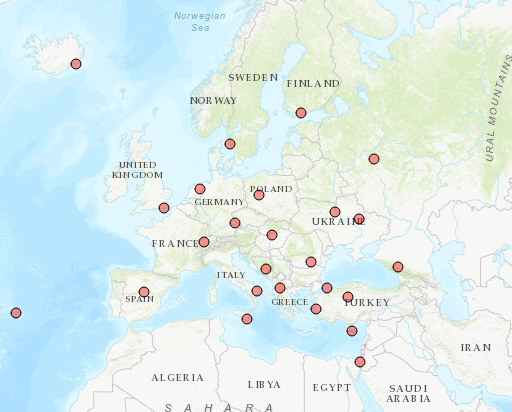
\includegraphics[width=0.8\textwidth]{igs.png}
            %\caption{Block diagram of a 1st order system.}
        \end{figure}
        \end{column}
        \begin{column}{.5\textwidth}
        \begin{figure}
            \centering
            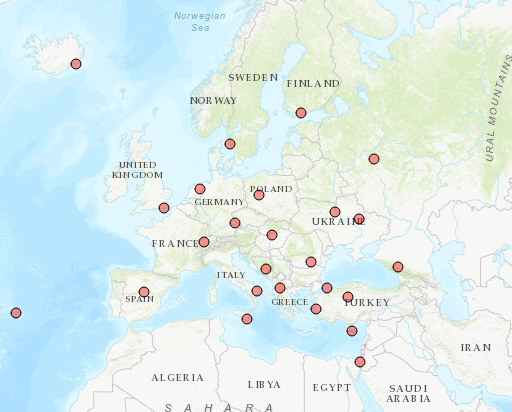
\includegraphics[width=0.9\textwidth]{igs.png}
            %\caption{Step response of a 1st order system.}
        \end{figure}
        \end{column}
    \end{columns}
\end{frame}
\note{}
